\documentclass[11pt,a4paper]{article}

\usepackage[T1]{fontenc}
\usepackage[utf8]{inputenc}
\usepackage[english]{babel}
\usepackage{lmodern}
%\usepackage{circuitikz}
\usepackage{color}
\usepackage{wrapfig}
\usepackage{placeins}
\usepackage{subfigure}
\usepackage{tabu}
\usepackage{fullpage}
\usepackage[squaren]{SIunits}
\usepackage{graphicx}
%\usepackage[pdftex]{graphicx}
\usepackage{epstopdf}
\usepackage{epsfig}
\usepackage{hyperref}
\usepackage{tikz}
\usepackage{tikz-qtree}
\usepackage{eurosym}
%\usepackage{chemist}
\usepackage{amsmath}
\usepackage{amssymb}
\usepackage{mathrsfs}
\usepackage{dsfont}% use $\mathds{1}$
\newcommand{\C}{\mathbb{C}}
\newcommand{\N}{\mathbb{N}}
\newcommand{\Z}{\mathbb{Z}}
\newcommand{\R}{\mathbb{R}}
\newcommand{\red}{\textcolor{red}}
\newcommand{\dis}{\displaystyle}
\newcommand{\dr}{\partial}
\newcommand{\txt}{\text}
\newcommand{\td}{\todo[inline]}
\newcommand{\ttt}{\texttt}
\newcommand{\itt}{\textit}

\usepackage{algorithm}
\usepackage{todonotes}
\usepackage[noend]{algpseudocode}

%\newtheorem{theoreme}			     {Théorème}	[chapter]
%\newtheorem{proposition}[theoreme]	 {Proposition}	
%\newtheorem{corollaire}	  [theoreme]	 {Corollaire}	
%\newtheorem{lemme}	      [theoreme]  {Lemme}		
%\newtheorem{definition}	         {Définition}[chapter]
%\theoremstyle{definition}
%\newtheorem{exemple}			     {Exemple}	[chapter]
%\newtheorem{contreexemple}[exemple]{Contre-exemple}
%\newtheorem{probleme}	             {Probl\`eme}[chapter]

\usepackage{listings}
\usepackage{textcomp}
\definecolor{listinggray}{gray}{0.9}
\definecolor{lbcolor}{rgb}{0.9,0.9,0.9}
\lstset{
	backgroundcolor=\color{lbcolor},
	tabsize=4,
	rulecolor=,
	language=matlab,
        basicstyle=\scriptsize,
        upquote=true,
        aboveskip={1.5\baselineskip},
        columns=fixed,
        showstringspaces=false,
        extendedchars=true,
        breaklines=true,
        prebreak = \raisebox{0ex}[0ex][0ex]{\ensuremath{\hookleftarrow}},
        frame=single,
        showtabs=false,
        showspaces=false,
        showstringspaces=false,
        identifierstyle=\ttfamily,
        keywordstyle=\color[rgb]{0,0,1},
        commentstyle=\color[rgb]{0.133,0.545,0.133},
        stringstyle=\color[rgb]{0.627,0.126,0.941},
}

\DeclareMathOperator{\e}{e}

\title{Titre}
\author{David Weicker}
\date{\today}

\begin{document}
\tabulinesep=1.2mm
\begin{center}
\hrule
\begin{tabular}{c}
\\[0.005cm]
\Large{SF2521: Homework Assignment 2}\\[0.3cm] %THIS IS THE TITLE
\textsc{Thomas} Garrett  \& \textsc{Weicker} David\\[0.2cm]
$\text{6}^{\text{th}}$ November 2015\\[0.2cm] %THIS IS THE DATE
\end{tabular}
\hrule
\end{center}

\section{Stability of Numerical Schemes}
We have the general scheme 
\begin{align*}
U^{n+1}  &= Q(t_n) U^n + \Delta t F^n \\
U^0 &= g
\end{align*}
where $U^n \in \mathbb{R}^d$. 

\subsection{Duhamel’s Principle}
We are given the following discrete Duhamel’s Principle:
\begin{align}
U^n = S_h(t_n,0)g+\Delta t \sum_{\nu = 0}^{n-1} S_h(t_n , t_{\nu + 1}) F^{\nu} , 
\end{align}
where $t_n = n \Delta t$, and 
\begin{align*}
S_h(t,t) &= I, \quad t \in \mathbb{R} \\
S_h(t_{n+1,t_{\mu}}) &= Q(t_n)S_h(t_n,t_{\mu}).
\end{align*}
\\
We begin by showing that (1) holds by induction.

Base Case: $n = 0$
\begin{align*}
U^0 &= S_h(0,0)g+\Delta t \sum_{\nu = 0}^{-1} S_h(0 , t_{\nu + 1}) F^{\nu} \\
& = 0
\end{align*}
which fits the general scheme. 
Now we assume that the (1) fits the general scheme at step $n$, and we want to show that this implies that it fits for step $n+1$.
\begin{align*}
U^{n+1} &= S_h(t_{n+1},0)g+\Delta t \sum_{\nu = 0}^{n} S_h(t_{+1}n , t_{\nu + 1}) F^{\nu} \\
&= Q(t_n)S_h(t_n,0)g + \Delta t Q(t_n) \sum_{\nu = 0}^{n-1} S_h(t_n , t_{\nu + 1}) F^{\nu} + S_h(t_{n+1} , t_{n + 1}) F^{n} \\ &= Q(t_n)(S_h(t_n,0)g + \Delta t \sum_{\nu = 0}^{n-1} S_h(t_n , t_{\nu + 1}) F^{\nu})+F^{n} \\ 
&= Q(t_n)U_n+F^{n} %\quad \text{by induction assumption} 
\end{align*}
which fits our general scheme.
\subsection{Bound in the $h$-norm}
We now wish to show that 
\begin{align*}
||S_h(t_{\nu+1},t_{\nu})||_h \leq Ke^{ah} \implies ||U^n||_h \leq K(e^{at_n} ||g||_h + \int_0^{t_n} e^{a(t_n-s)} ds \max_{0\leq \nu \leq n-1} ||F^{\nu}||_h
\end{align*}
Taking $||\cdot ||_h$ of both sides of (1), then by Cauchy-Schwartz inequality, we have
\begin{align*}
||U^n||_h &= ||S_h(t_n,0)g+\Delta t \sum_{\nu = 0}^{n-1} S_h(t_n , t_{\nu + 1}) F^{\nu} ||_h \\
&\leq ||S_h(t_n,0)||_h||g||_h+||\Delta t||_h \sum_{\nu = 0}^{n-1} ||S_h(t_n , t_{\nu + 1})||_h || F^{\nu} ||_h \\
&\leq Ke^{at_n}||g||_h+||\Delta t||_h \sum_{\nu = 0}^{n-1} ||S_h(t_n , t_{\nu + 1})||_h || F^{\nu} ||_h\\
&\leq Ke^{at_n}||g||_h+\Delta t \sum_{\nu = 0}^{n-1} Ke^{a(t_n - t_{\nu+1})} || F^{\nu} ||_h\\ 
\text{we notice that} \enspace & \Delta t \sum_{\nu = 0}^{n-1} Ke^{a(t_n - t_{\nu+1})} \enspace \text{is a right Remman sum of a strictly decreasing function, thus} \\
&\leq Ke^{at_n}||g||_h+ K\int_0^{t_n} e^{a(t_n - s)} ds || F^{\nu} ||_h\\ 
&\leq K(e^{at_n}||g||_h+ \int_0^{t_n} e^{a(t_n - s)} ds \max_{0\leq \nu \leq n-1} ||F^{\nu}||_h)
\end{align*}
IS a POSITIVE??
\subsection{a Value}
If $a = h^{-1/2}$, then we would have $||S_h(t_{\nu + 1}, t_{\nu})||_h \leq Ke^{\sqrt{h}}$. Plugging this into our second inequality, we obtain, 
\begin{align*}
||U^n||_h\leq K(e^{\sqrt{t_n}}||g||_h+ \int_0^{t_n} e^{\sqrt{t_n - s}} ds \max_{0\leq \nu \leq n-1} ||F^{\nu}||_h)
\end{align*}

\section{Shallow water model}
bla
The shallow water equation can be written in quasilinear form as \begin{align*}
u_t + f'(u) u_x = 0
\end{align*}
where $ u = (h,hv)^T $,
\begin{align*}
f'(u) = \begin{pmatrix}
0 & 1 \\
-(\frac{u_2}{u_1})^2 + gu_1 & 2 (\frac{u_2}{u_1})
\end{pmatrix}
\end{align*}
and 
\begin{align*}
q(x,0) &= \begin{pmatrix}
H + \epsilon e^{-(x-L/2)^2/w^2} \\
0
\end{pmatrix} 
\end{align*}
Now, to make this system linear we must simply pick a constant state $(h_0,v_0)$ which is consistent with the boundary and initial conditions. We choose $(h_0,v_0)$ at $x=0$ and $t=0$. We can now compute $(h_0,v_0)$ using the initial condition. We get $(h_0,v_0) \approx (1,0)$. Thus we have 
\begin{align*}
f'(u) = \begin{pmatrix}
0 & 1 \\
g & 0
\end{pmatrix} = \begin{pmatrix}
0 & 1 \\
9.61 & 0
\end{pmatrix}
\end{align*}
We can see easily $f'(u)$ has eigenvalues $\lambda_{1,2} = \pm \sqrt{9.61} = \pm 3.1$ which are real. It also has a full set of eigenvectors i.e. $(1,3.1)^T$ and $(-1,3.1)$. This together confirm that the linear problem is hyperbolic. We also know that the wave speeds are the eigenvalues, so we have wave speeds $\pm \sqrt{9.61}$

\subsection{Analytical Solution}
We have the PDE, 
\begin{align*}
q_t + f'(u) q_x = 0
\end{align*}
which we have shown can be written as 
\begin{align*}
q_t + V D V^{-1} q_x &= 0 \\
\implies V^{-1} q_t + D V^{-1} q_x &= 0
\end{align*}
where 
\begin{align*}
 V = \begin{pmatrix}
1 & -1 \\
3.1 & 3.1
\end{pmatrix}, D= \begin{pmatrix}
3.1 & 0 \\
0 & -3.1
\end{pmatrix},  \text{and} V^{-1} = \begin{pmatrix}
0.5 & 0.1613 \\
-0.5 & 0.1613
\end{pmatrix}
\end{align*} and initial condition
\begin{align*}
q(x,0) &= \begin{pmatrix}
H + \epsilon e^{-(x-L/2)^2/w^2} \\
0
\end{pmatrix} 
\end{align*}
Now, defining a new variable $r = V^{-1} q$ we have the decoupled system of equations
\begin{align*}
r_t + Dr_x = 0
\end{align*}
and 
\begin{align*}
r(x,0) = V^{-1} q(x,0) = \frac{1}{2} \begin{pmatrix}
H + \epsilon e^{-(x-L/2)^2/w^2} \\
-H - \epsilon e^{-(x-L/2)^2/w^2}
\end{pmatrix} 
\end{align*}
From Lavengen, we know the solutions of this system are 
\begin{align*}
	r_1(x,t)&=r_1(x+\lambda_1t,0)=\frac{1}{2} (H + \epsilon e^{-(x+3.1t-L/2)^2/w^2}) \\
	\text{and} \quad r_2(x,t)&=r_2(x+\lambda_2t,0)= \frac{1}{2}(-H - \epsilon e^{-(x-3.1t-L/2)^2/w^2})
\end{align*} 
Finally switching back to $q$, we get 
\begin{align*}
q(x,t) = Vr(x,t) &= \frac{1}{2} \begin{pmatrix}
H + \epsilon e^{-(x+3.1t-L/2)^2/w^2} +H + \epsilon e^{-(x-3.1t-L/2)^2/w^2} \\
3.1(H + \epsilon e^{-(x+3.1t-L/2)^2/w^2} -H - \epsilon e^{-(x-3.1t-L/2)^2/w^2})
\end{pmatrix} \\
&= \frac{1}{2}\begin{pmatrix}
 2H + \epsilon e^{-(x+3.1t-L/2)^2/w^2} + \epsilon e^{-(x-3.1t-L/2)^2/w^2} \\
3.1( \epsilon e^{-(x+3.1t-L/2)^2/w^2} - \epsilon e^{-(x-3.1t-L/2)^2/w^2})
\end{pmatrix}
\end{align*} 
Now, simply plugging in $t=1$ we get
\begin{align*}
q(x,1) = \frac{1}{2}\begin{pmatrix}
 2H + \epsilon e^{-(x+3.1-L/2)^2/w^2} + \epsilon e^{-(x-3.1-L/2)^2/w^2} \\
3.1( \epsilon e^{-(x+3.1-L/2)^2/w^2} - \epsilon e^{-(x-3.1-L/2)^2/w^2})
\end{pmatrix}
\end{align*}

\subsection{Numerical Solution of the Linear Problem}
To compare the results from the non-linear and linear problems, we compare the numerical solutions of the problems using the same method. The code for the numerical solution of the linear problem is almost exactly the same as for the linear problem, except the flux $f$. For the linear problem we compute the flux function from the information above. 
\begin{align*}
f'(u) = \begin{pmatrix}
0 & 1 \\
g & 0
\end{pmatrix} \rightarrow 
f(u) = \begin{pmatrix}
u_2 \\
gu_1
\end{pmatrix}
\end{align*}
\subsection{Non-reflecting boundary conditions}
Finally, we are going to apply non reflecting conditions at the boundaries. As explained in Leveque chapter 7, we extrapolate the variables at the ghost cells by saying :
\begin{align*}
h_0 &= h_1\\
h_N &= h_{N+1}\\
v_0 &= v_1 \implies hv_0 = hv_1\\
v_N &= v_{N+1} \implies hv_N = hv_{N+1}
\end{align*}

Intuitively, the flow is going to "go out" of the domain with such boundary conditions.

The code is available at the end of the report. The structure does not change much, the only difference is the computations of the values of the ghost cells.

Figure \ref{noRe} shows the results when applying the extrapolation for the ghost cells. We can see that at first nothing changes from the original problem. This is coherent since we only changed the boundary conditions . But the waves go out of the domain when reaching the boundaries. This is exactly what we wanted ! There is no reflection noticeable. To investigate a bit more, we can compute the integral of the height on the domain. At $t=2.1$, this value is 10 with accuracy up to floating point errors so we can be sure that there is no reflection at all.

\begin{figure}
\begin{center}
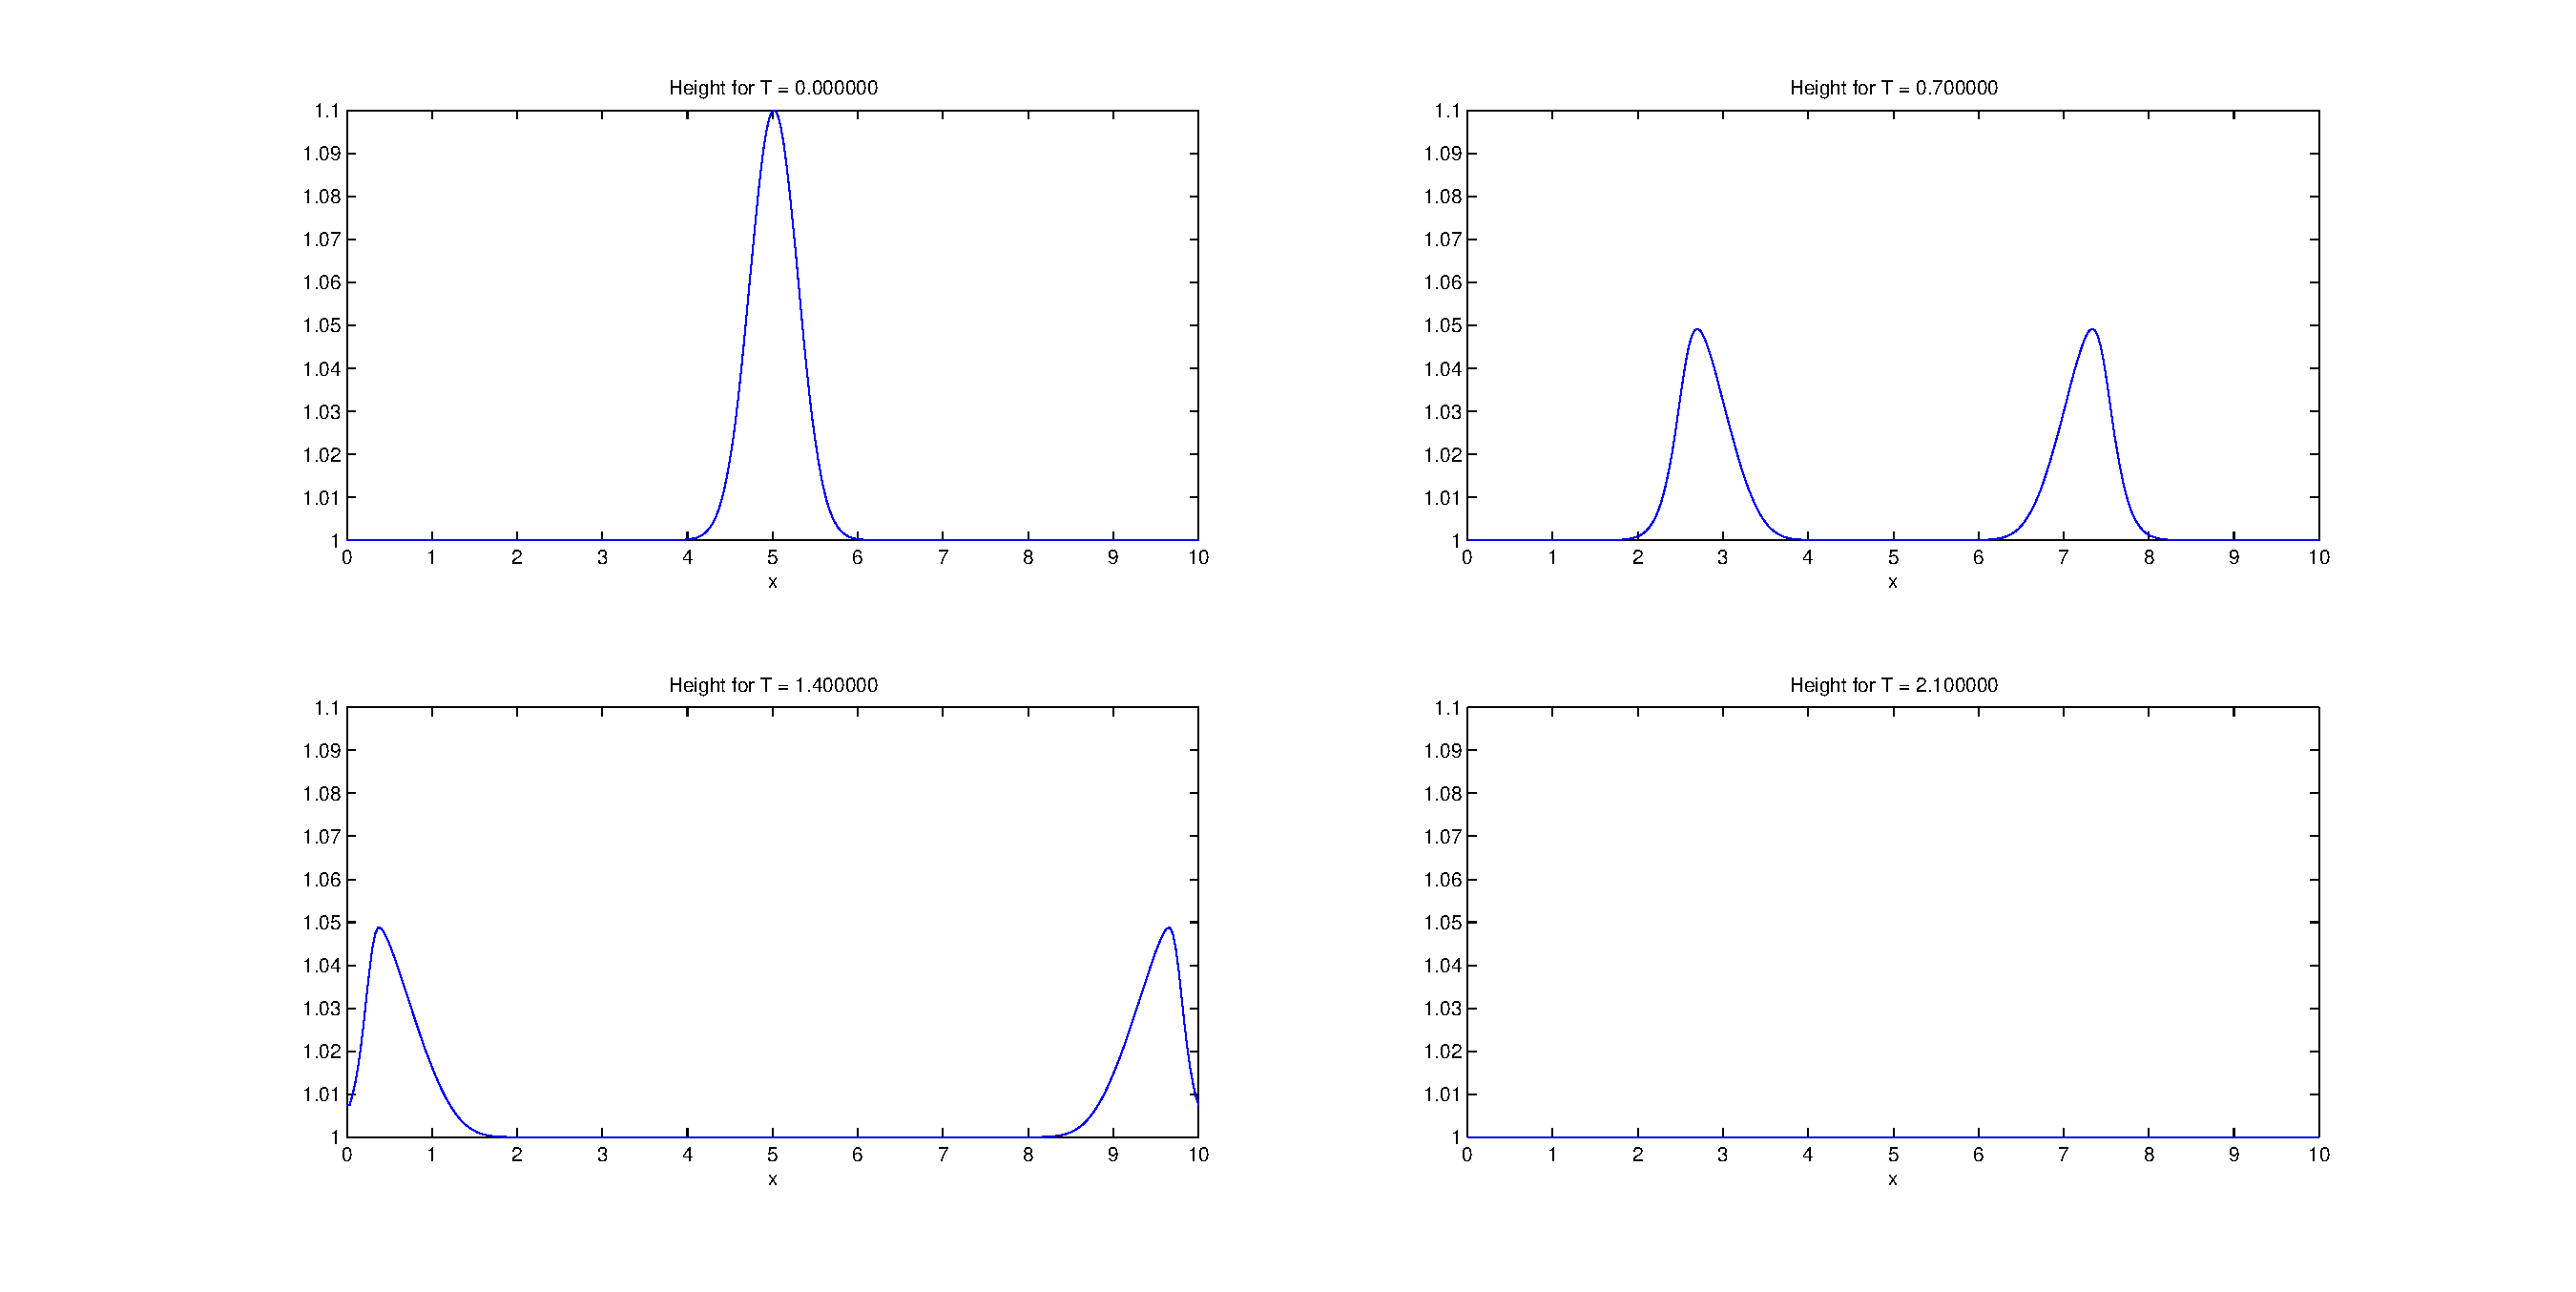
\includegraphics[scale=0.4]{noRe.eps}
\caption{Results with non reflective boundary conditions}
\label{noRe}
\end{center}
\end{figure} 

\end{document}